\section{Experimental Results}
\subsection{Fitting Results}

For each of the Twitter datasets, we were interested in quantifying the transitions of users through the different compartments of the SIS and SEIZ models.
%\narenc{Figure references are wrong! Please do not hardwire figure numbers.}
%,~\ref{fig:Benedict},~\ref{fig:Gas_explosion},~\ref{fig:Michelle},~\ref{fig:Obama},~\ref{fig:Doomsday},~\ref{fig:Castro},
Figures~\ref{fig:Boston_bombing} -~\ref{fig:Mexico_riot} display the results for the best fit of SIS and SEIZ models (Equations~\ref{eq:sis} and~\ref{eq:seiz}) to the eight Twitter stories. Also displayed for each figure are the relative error in 2-norm $$\frac{||I(t) - tweets(t)||_2}{||tweets(t)||_2}$$ and the mean error deviation $$\frac{\sum_{i=1}^n|I(t_i)-tweets(t_i)|}{n},$$  where $n$ is the number of data points.

The error metrics for these eight stories clearly indicate that the SEIZ model fits the Twitter data much more accurately than the SIS model. Furthermore, the low relative error of the SEIZ model fit suggests that this model accurately represents the Twitter data for each of the eight stories; see Table~\ref{table:error}. A common observation about all the eight stories is that the SEIZ model is far more accurate in modelling the initial spread of the news on Twitter as compared with the SIS model. This behaviour can be explained by the delay caused by individuals in the ``Exposed" category taking some time before posting a story themselves~\cite{powerofgoodidea:2006}.

Given that the SEIZ model is superior to the SIS model in this application, and that the SEIZ model demonstrates an accurate representation of information diffusion on Twitter, a natural question arises ``How can this model help us?" The answer is really simple. Since we have a mathematical model for the Twitter data, we can study solutions to some of the constraints as mentioned in the ``Practical Issues" section. A well fitted SEIZ model provides values for all contact rates and transition probabilities as defined by Equation~\ref{eq:seiz}. These parameters empower us to investigate the dynamics of news and rumor spread on Twitter in a fashion that is not possible without a mathematical model. Table~\ref{table:parameters} specifies the SEIZ model parameters that we can now examine to assess news and rumor propagation on Twitter.



\begin{figure*}[t]
\centering
\subfigure[Boston]{
   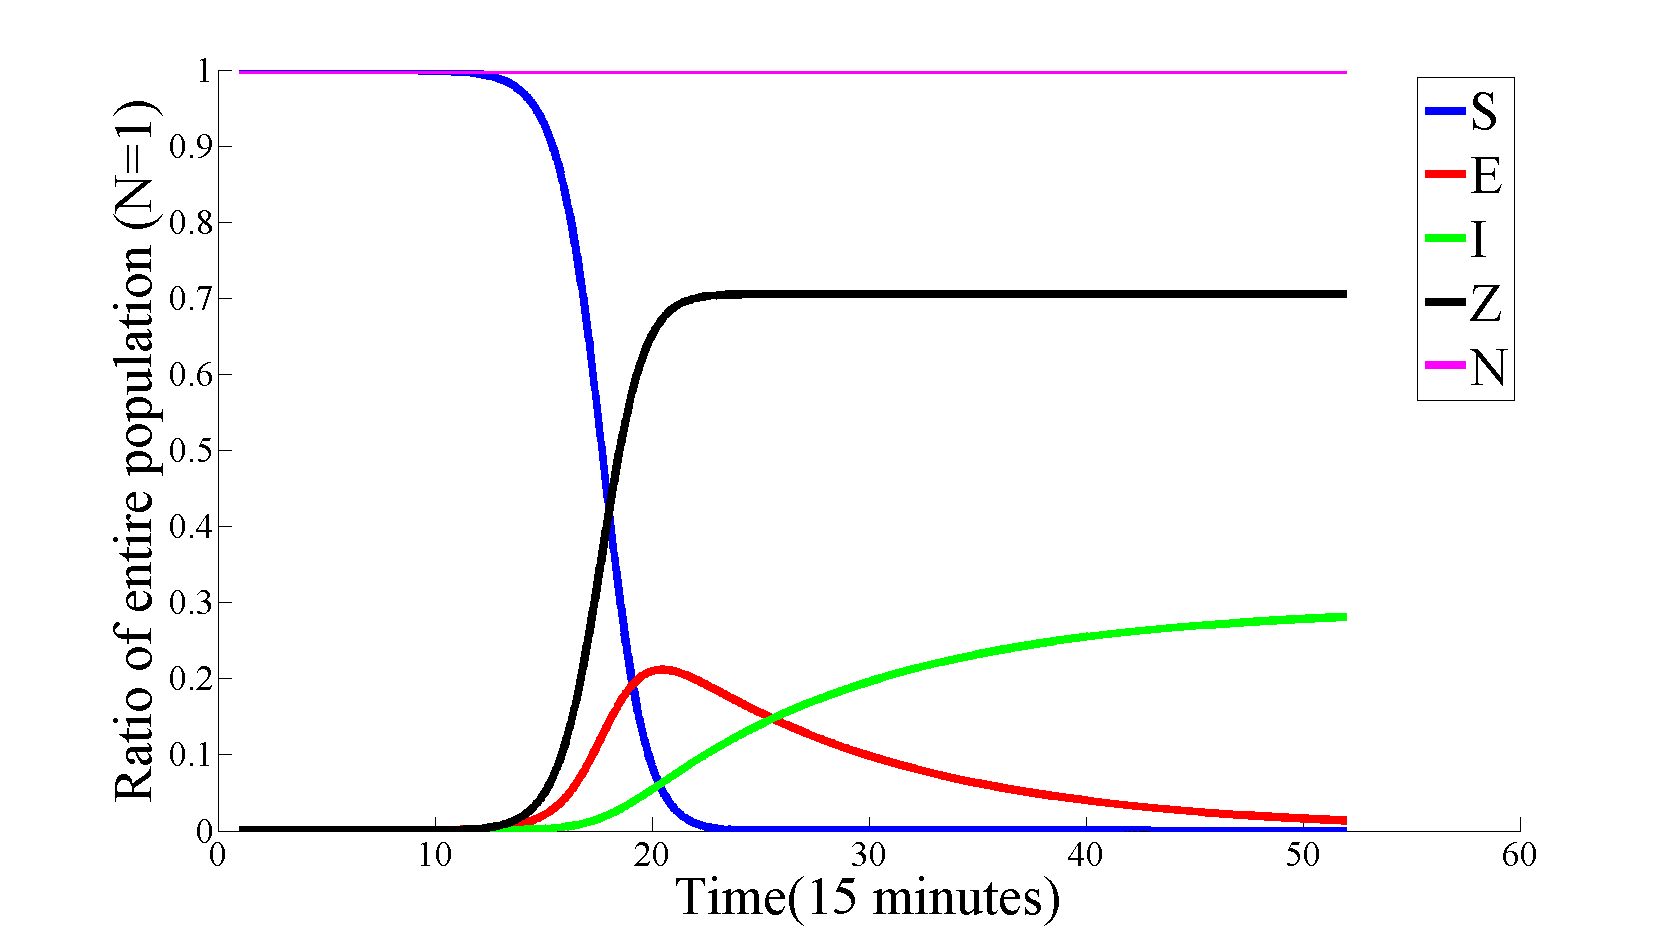
\includegraphics[width=2in,height=1.5in] {pictures/Boston_SEIZ_total.png}
  \label{fig:Boston_time}
 }
  \subfigure[Pope]{
   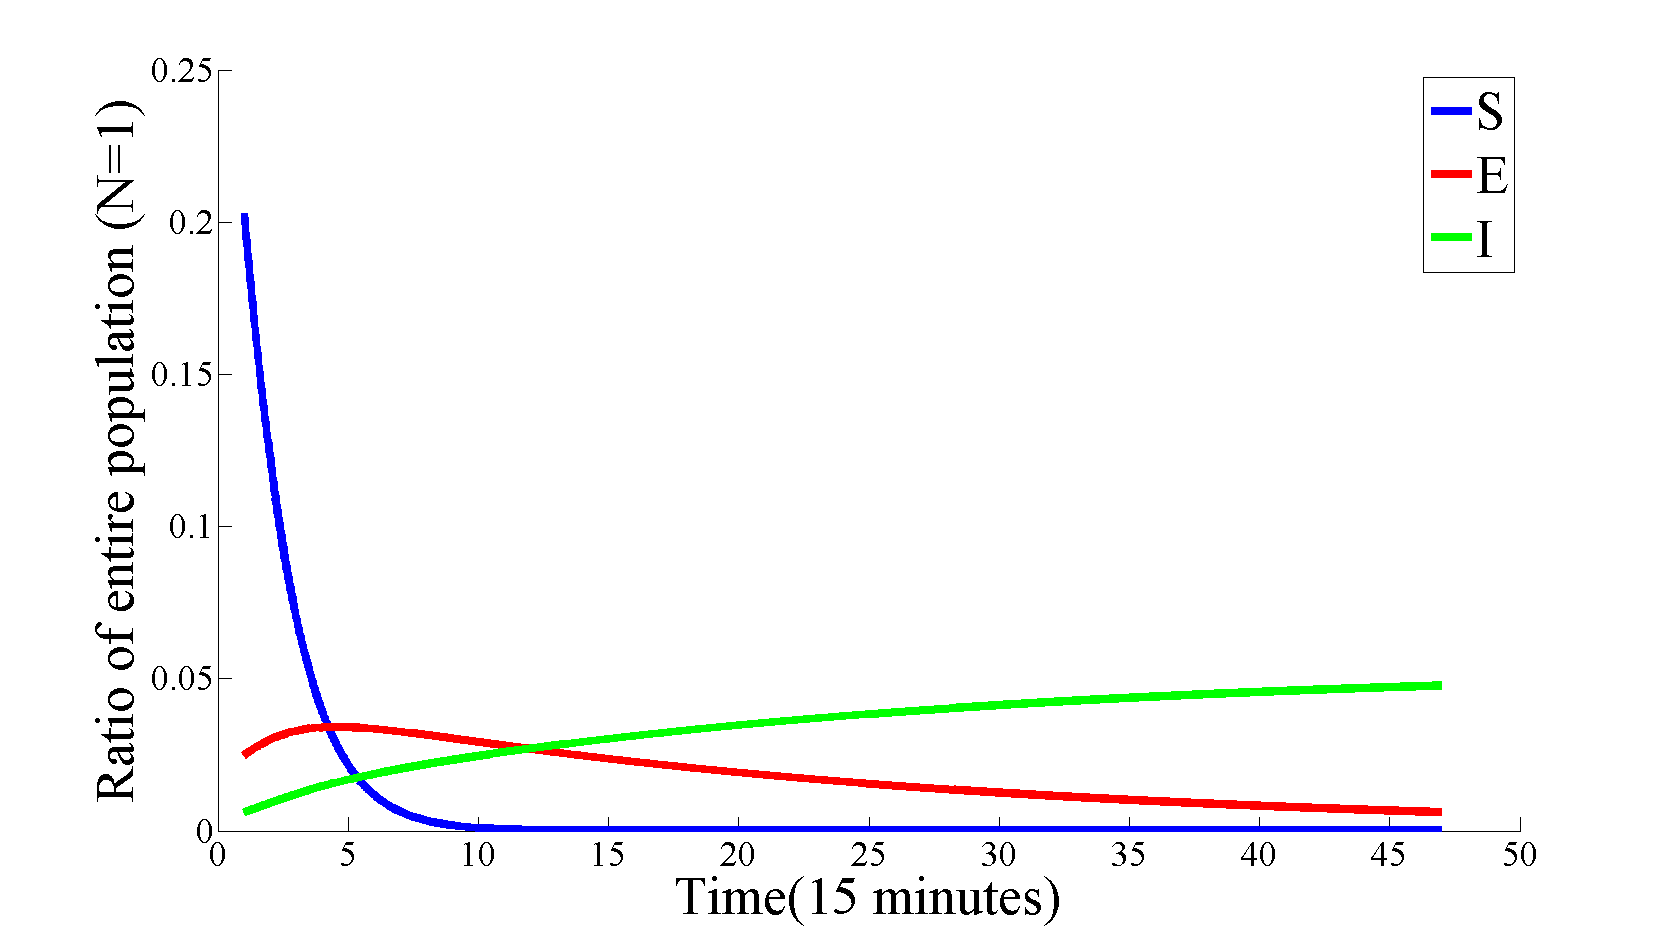
\includegraphics[width=2in,height=1.5in] {pictures/Pope_SEIZ_total.png}
   \label{fig:Pope_time}
 }
  \subfigure[Amuay]{
   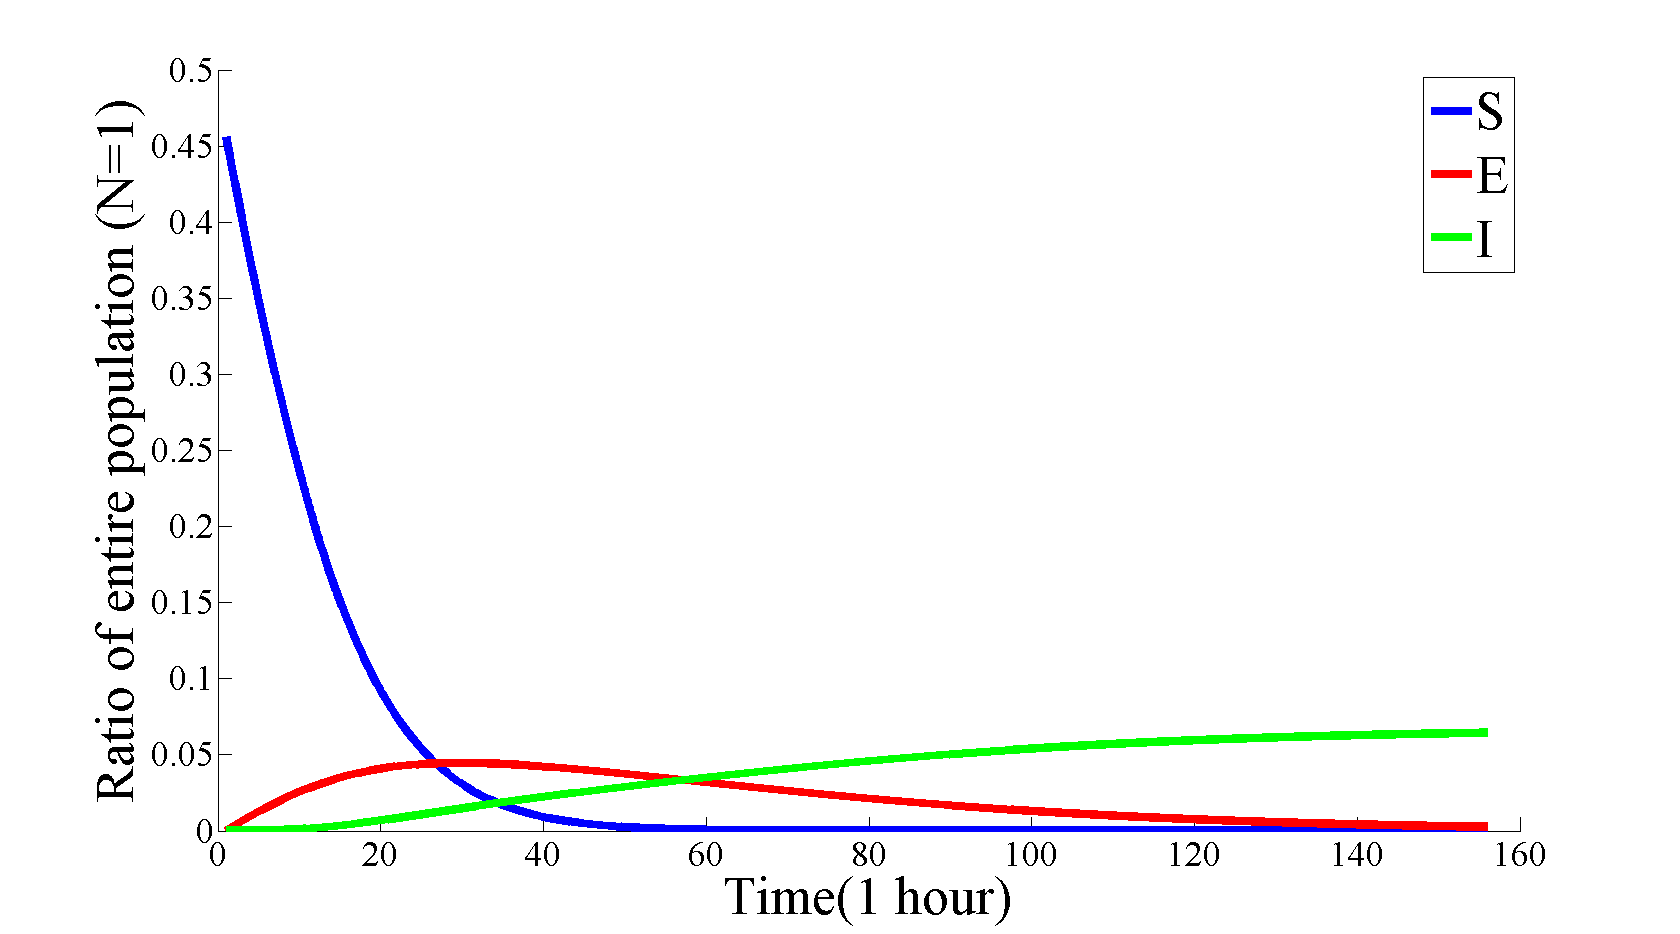
\includegraphics[width=2in,height=1.5in] {pictures/Amuay_SEIZ_total.png}
   \label{fig:Gas_time}
 }
\subfigure[Michelle]{
   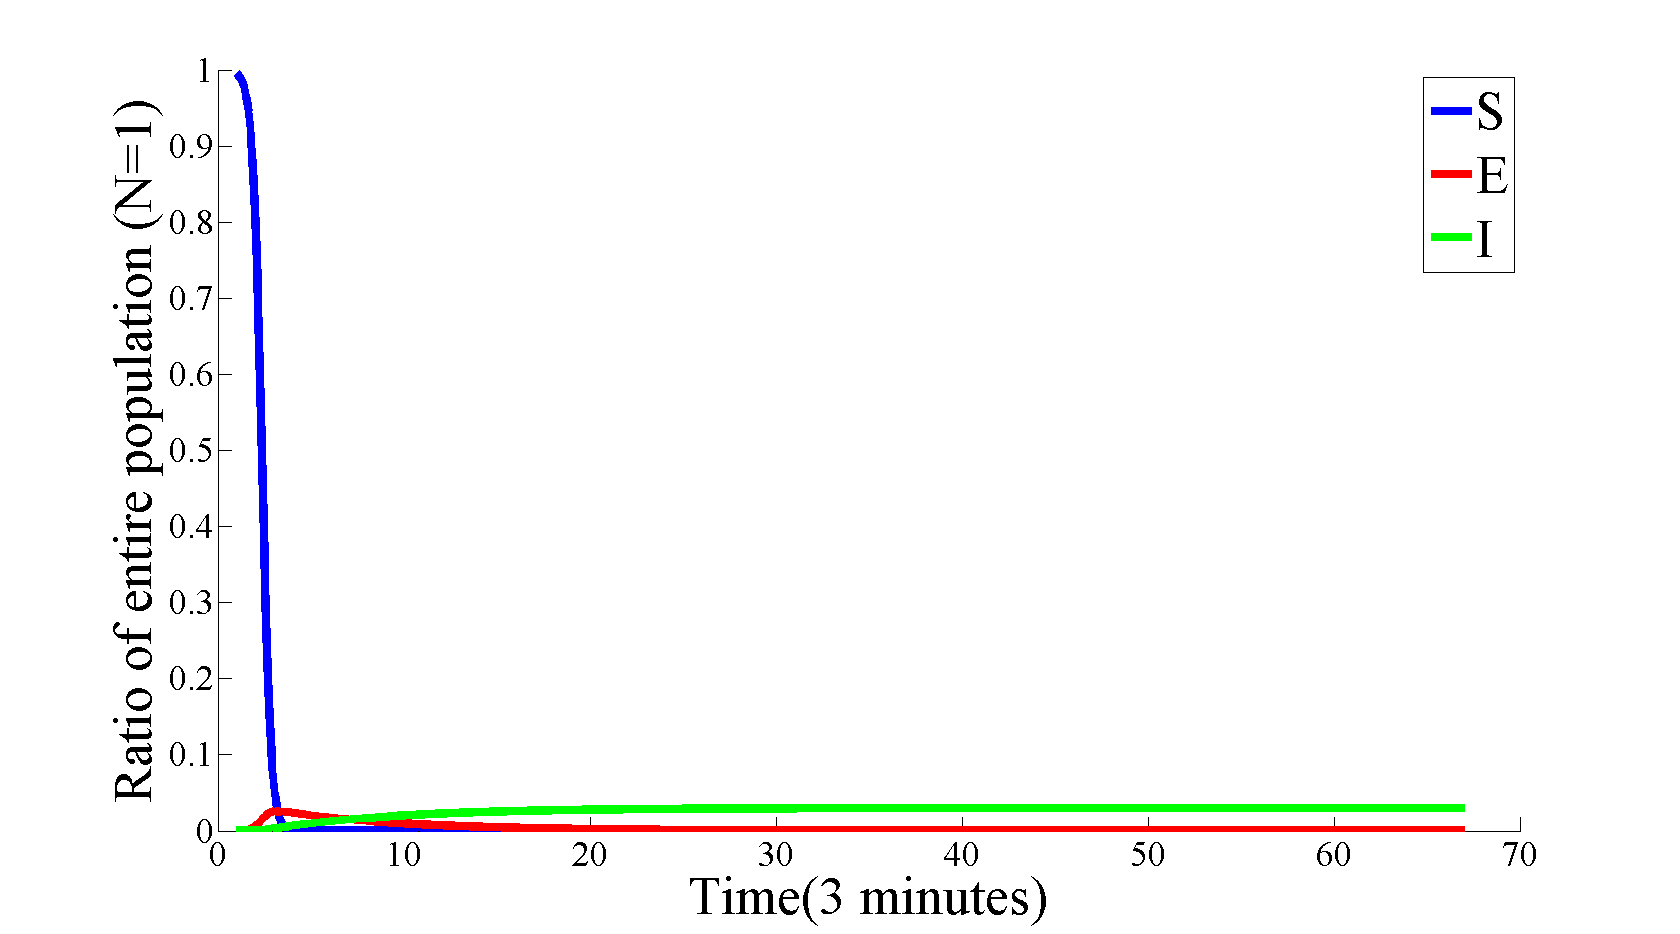
\includegraphics[width=2in,height=1.5in] {pictures/Michelle_SEIZ_total.png}
  \label{fig:Michelle_time}
 }
  \subfigure[Obama]{
   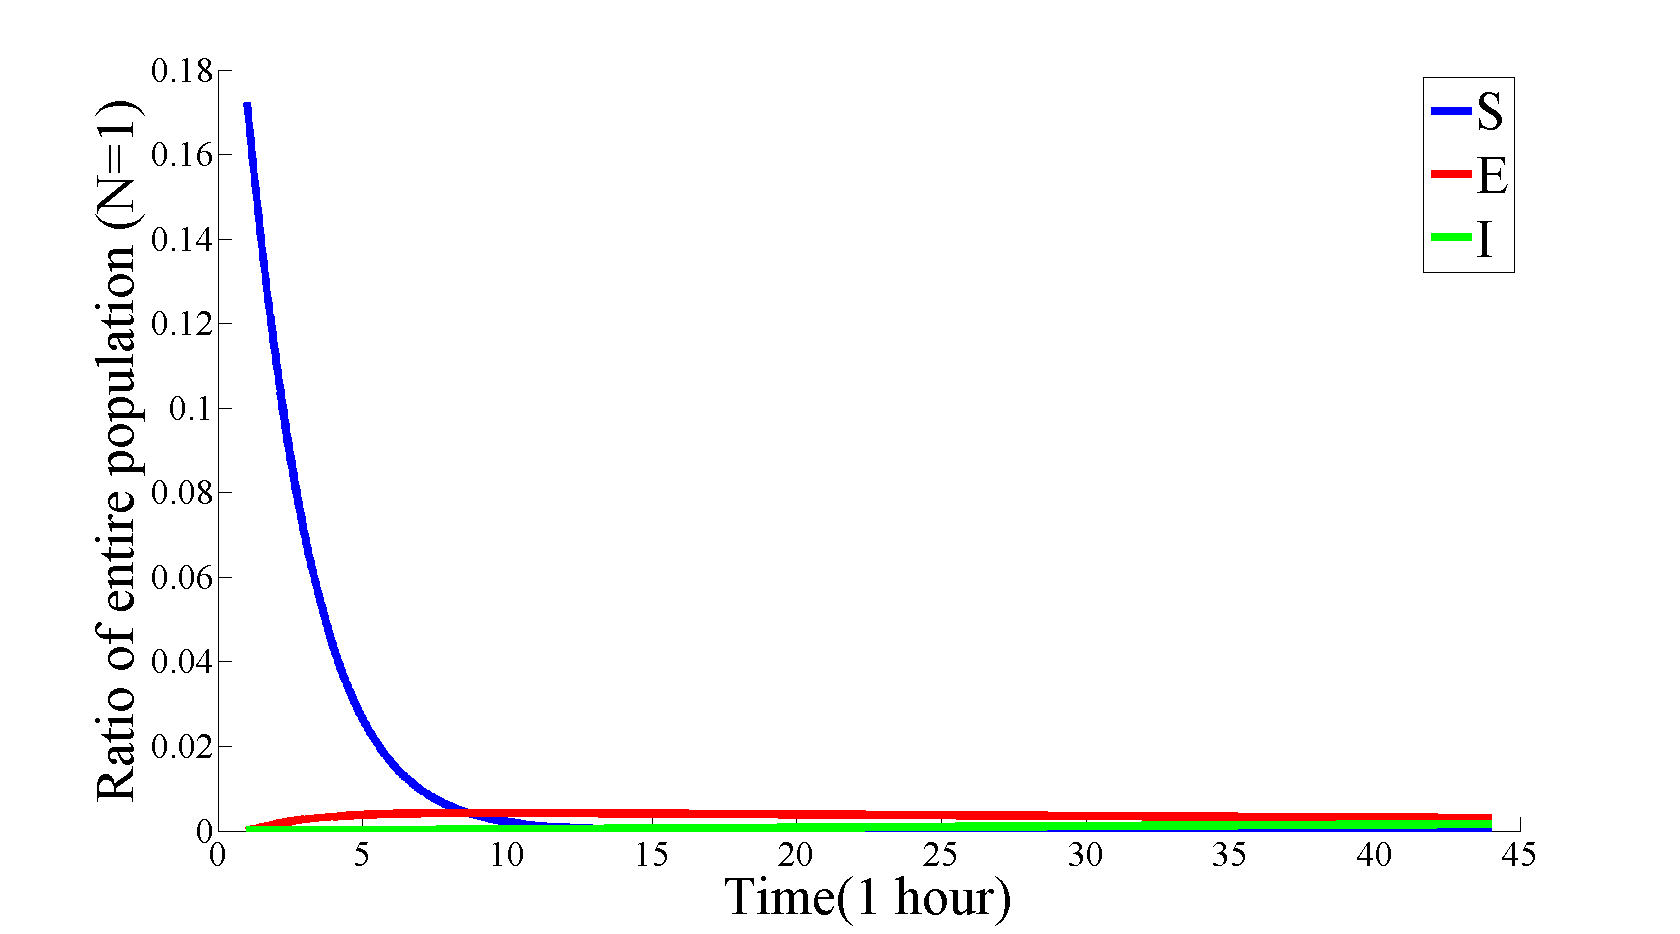
\includegraphics[width=2in,height=1.5in] {pictures/Obama_SEIZ_total.png}
   \label{fig:Obama_time}
 }
  \subfigure[Doomsday]{
   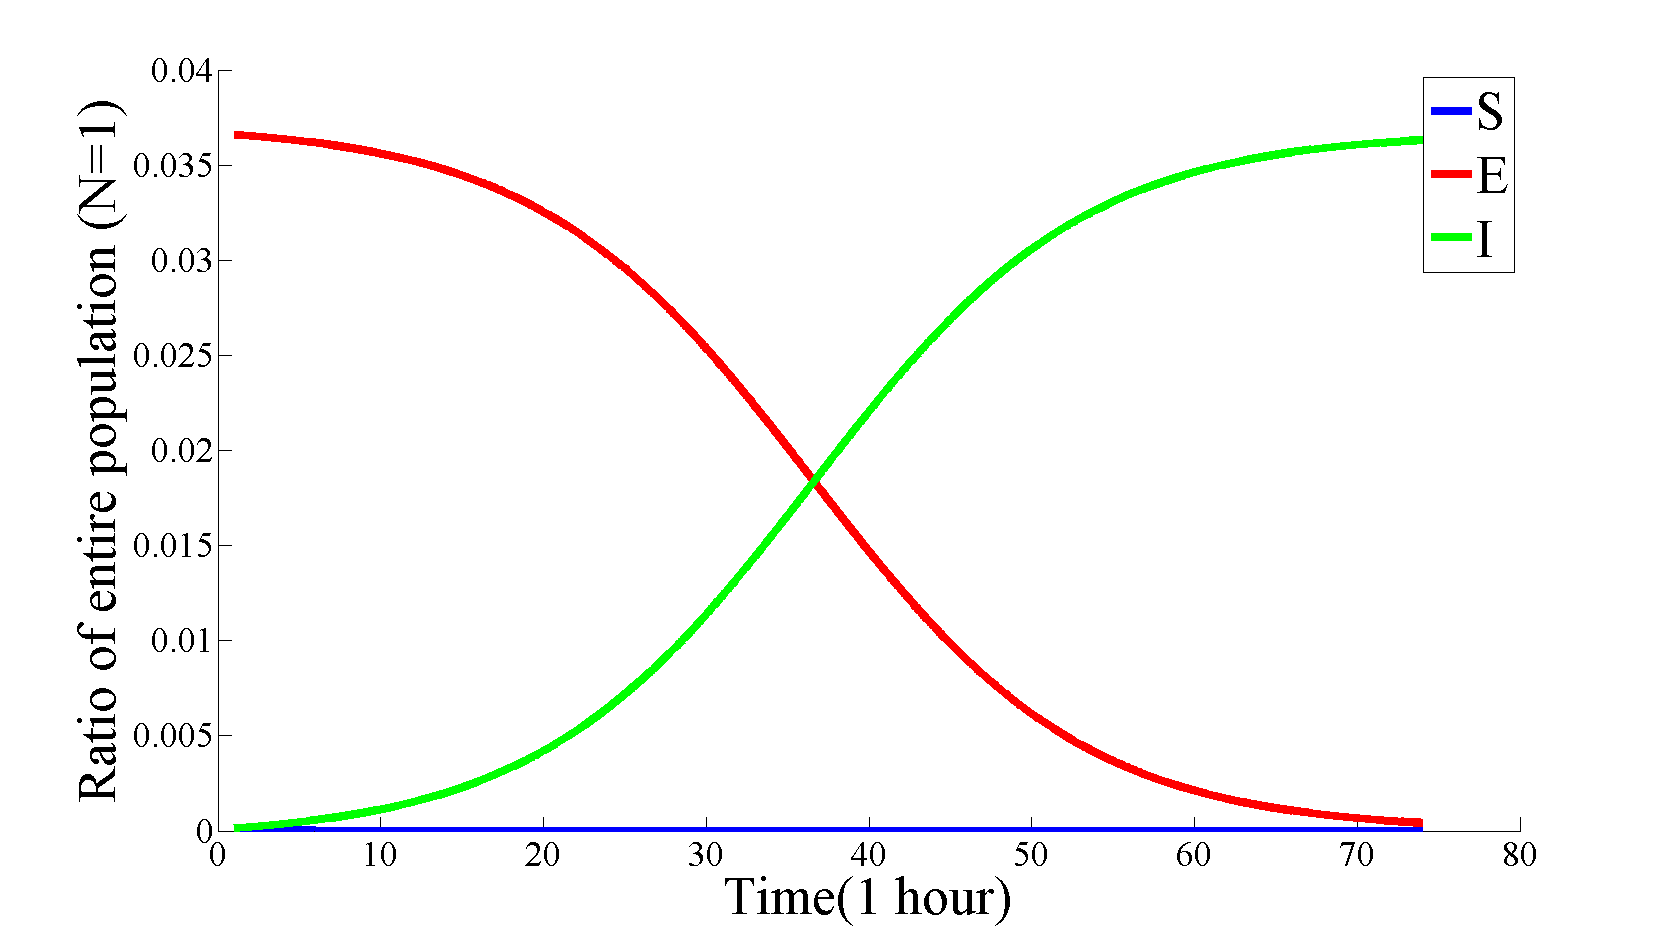
\includegraphics[width=2in,height=1.5in] {pictures/Doom_SEIZ_total.png}
   \label{fig:Doomsday_time}
 }
   \subfigure[Castro]{
   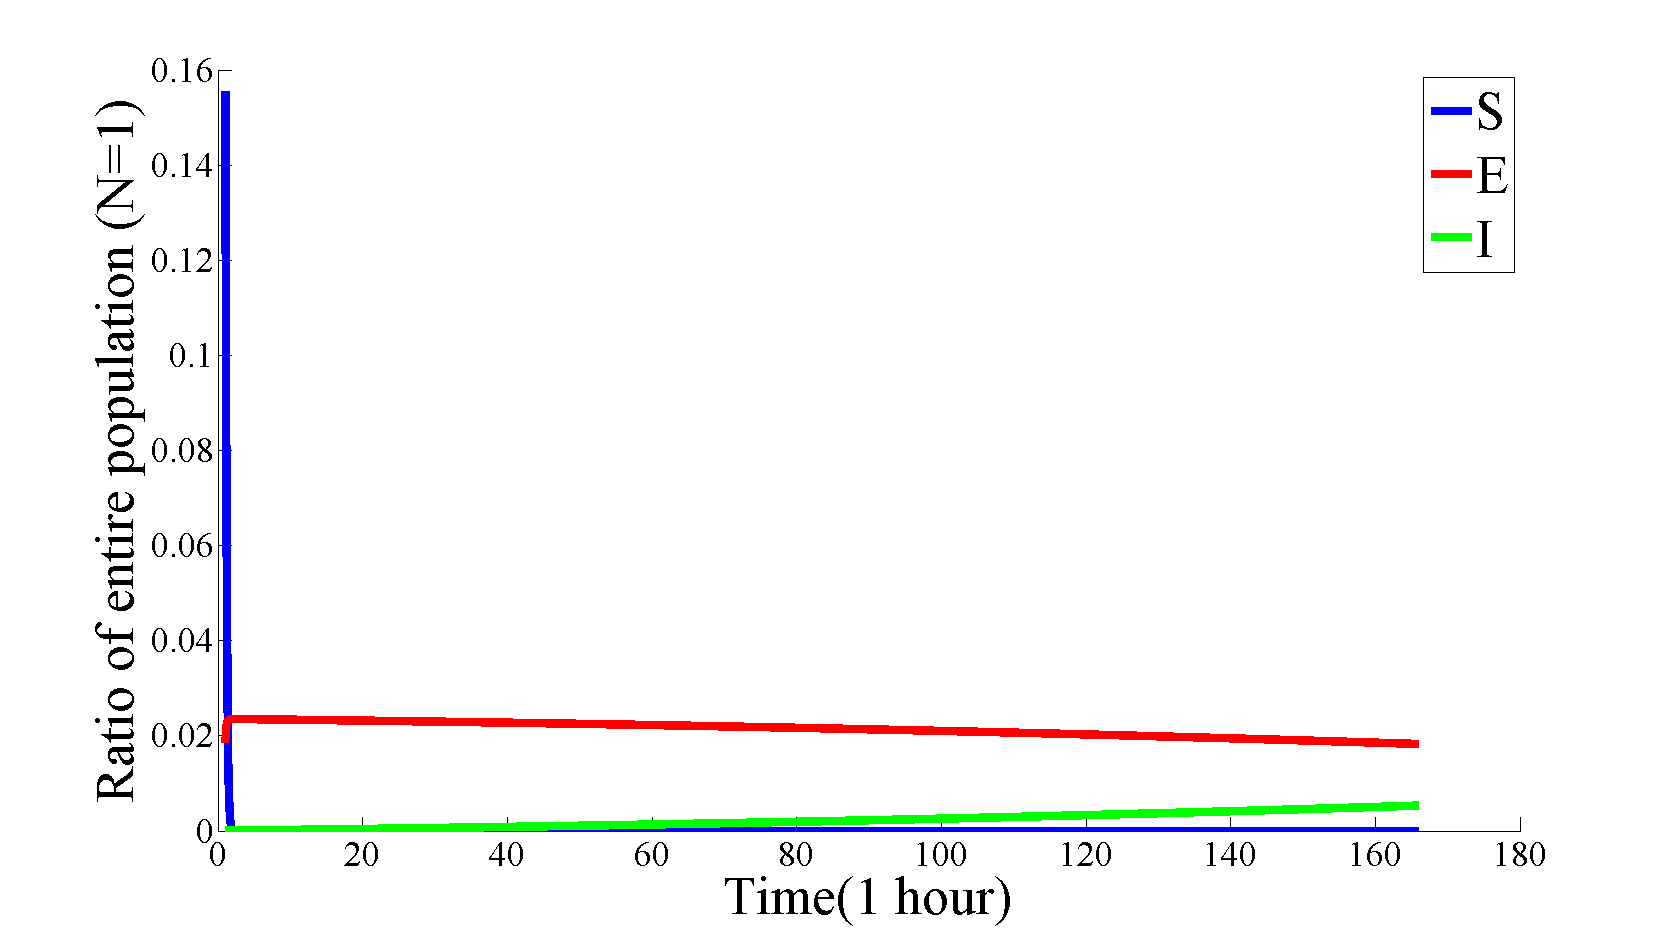
\includegraphics[width=2in,height=1.5in] {pictures/Castro_SEIZ_total.png}
  \label{fig:Castro_time}
 }
 \subfigure[Riot]{
   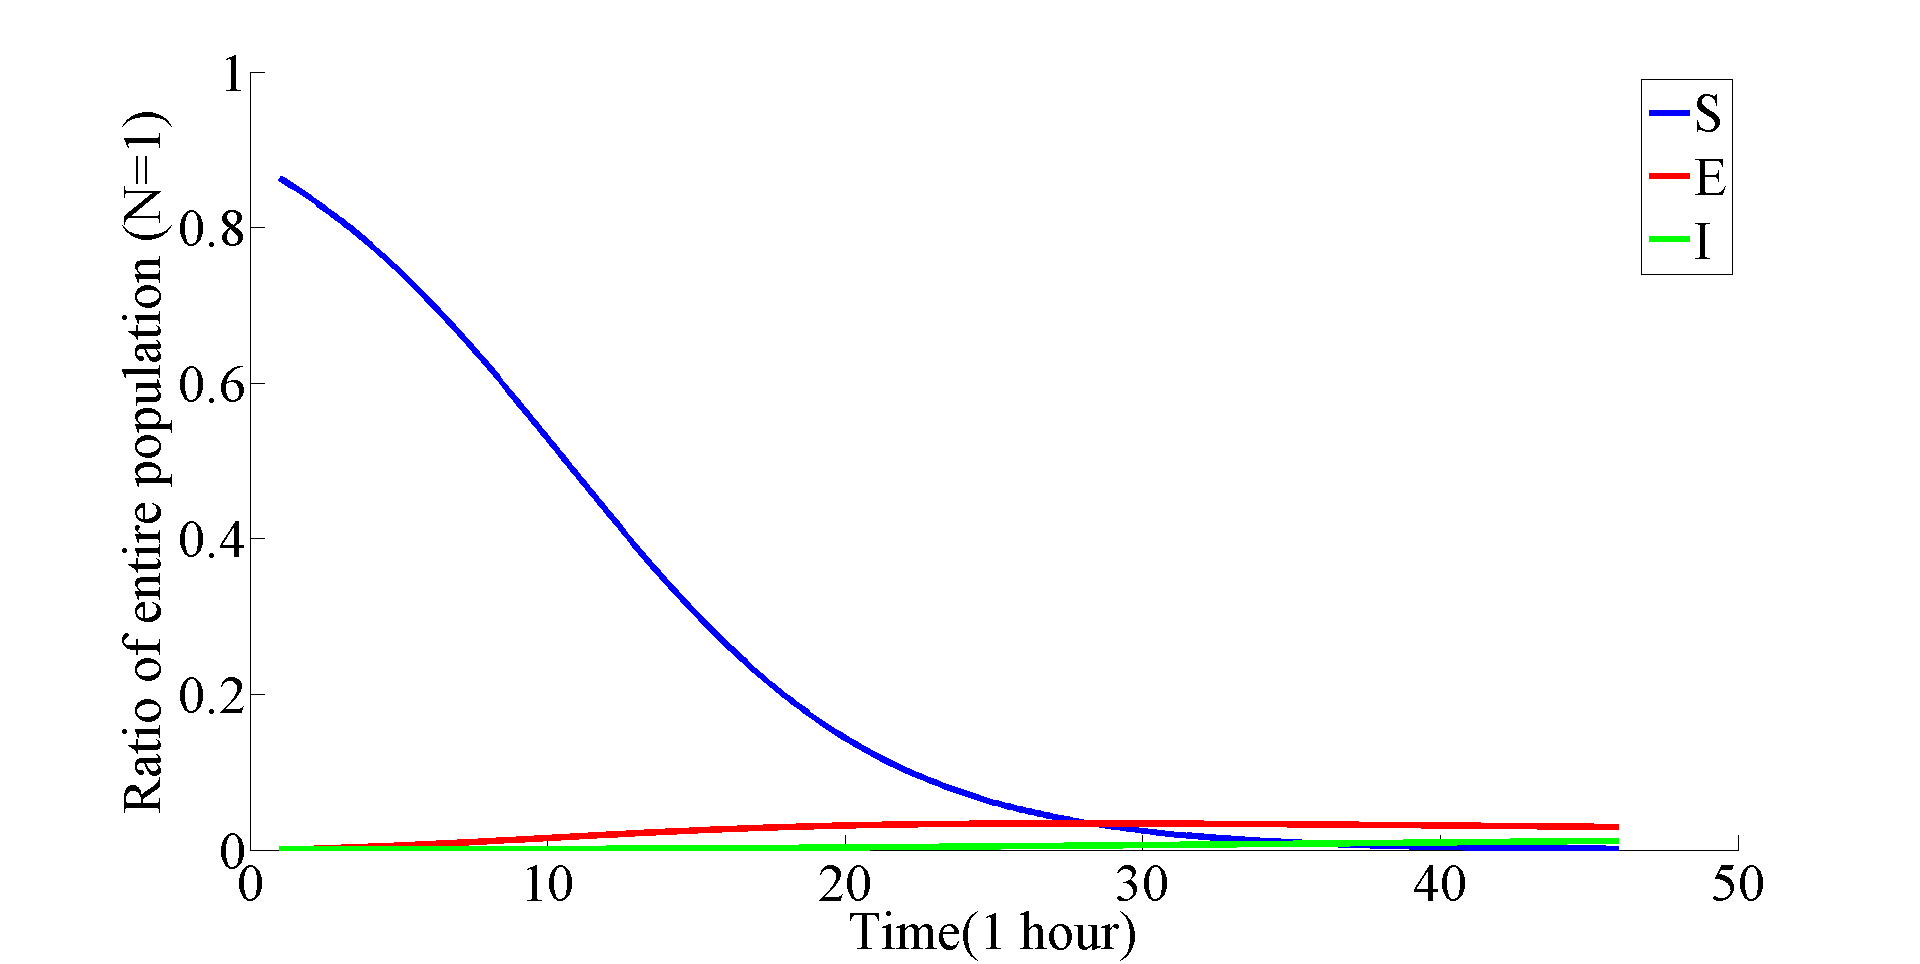
\includegraphics[width=2in,height=1.5in] {pictures/Riot_SEIZ_total.png}
  \label{fig:Mexico_time}
 }
\vspace{-0.5em}
\caption{SEIZ compartment time-course results.
\label{fig:Time_course}
}
\end{figure*}


\subsection{Boston Marathon Bombing Analysis}

To demonstrate a line of analysis that is now possible with the SEIZ mathematical model, we use quantities from the SEIZ model fit of the Boston Marathon bombing Twitter data (Table~\ref{table:parameters}). Results are summarized in Table~\ref{tab:seiz_boston_bombing}.

Here we discuss the dynamics of all 4 compartments, so we specially show all 4 compartments in the SEIZ time-course plot only for Boston Marathon bombing (Figure~\ref{fig:Boston_time}). These results suggest that the effective rate of susceptible individuals becoming skeptics is much greater than those that becoming infected. The decrease in $S(t)$ occurs directly with an increase in $Z(t)$, and $S(t)$ becomes stable at the same time that $Z(t)$. $I(t)$ does increase as $S(t)$ decreases, but its rate of change is much slower, and the majority of $I(t)$ increase occurs after $S(t)$ has stabilized to a minimal value, demonstrating that the continued change in the infected compartment has no further influence on the change in the susceptible compartment.

Table~\ref{tab:seiz_boston_bombing} also demonstrates that the skeptics compartment is more influential on transitioning susceptible users to the exposed class than does infected users. Figure~\ref{fig:Boston_time} shows this as the increase in $E(t)$ is strongly correlated with the increase in $Z(t)$. $E(t)$ also peaks as $Z(t)$ peaks, and $E(t)$ begins to decrease at a rate negative to that of the $I(t)$ increase. In fact, the increase in $I(t)$ directly coincides with a comparable decrease in $E(t)$. These data suggest that the increase in infected users is not due in large part by recruitment of susceptible users, but rather from the natural transition to the infected compartment by exposed individuals.

Putting this all together, we can deduce that virtually all individuals are initially in the susceptible compartment. Most susceptible users become skeptics from interaction with skeptics, and those susceptible users that do transition to the exposed class do so by their interaction with skeptics. The infected compartment increases predominately from the exposed class, and not from direct recruitment of susceptible individuals. Thus, these findings suggest that it was in-fact non-Twitter mediums that most greatly aided in the generation of Twitter propagation! Further, the $\frac{\epsilon}{\rho}$ ratio indicates that the exposed users became infected more so due to information incubation and self-adoption, and not so much from direct contact with infected users.

\begin{table}
\renewcommand{\arraystretch}{2.5}
\small
\centering
\caption{Ratios of SEIZ model for Boston dataset.}
\vspace{0.5em}
\begin{tabular}{|p{2.5cm} |  p{1.5cm}|} \hline
$\displaystyle \frac{bl}{\beta p}$ & 3.1E5\\ \hline
$\displaystyle \frac{b(1-l)}{\beta (1-p)}$ & 1.0E4 \\ \hline
$\displaystyle \frac{\epsilon}{\rho}$ & 7.8\\
\hline\end{tabular}
\label{tab:seiz_boston_bombing}
\end{table}

% I added this sentence to answer review 1.4
The remaining instances of SEIZ time-course plots are shown in Figure~\ref{fig:Time_course}, we can see how S, E, and I dynamic change over time. These analyses exemplify the types of analyses that can be used to study Twitter dynamics via the SEIZ population model.

\subsection{Rumor Detection}
We next examined if our implementation of the SEIZ model, applied to our Twitter examples, could be utilized to facilitate the discrimination of true news from rumors. We began by assembling an equation to relate the key parameters of the SEIZ model. In our first attempt at performing this, we restricted our attention to the exposed compartment; this class has direct or indirect interconnections between the other three compartments, and is a key path to the infected compartment. To exemplify this, consider the extreme case where susceptible individuals are attempted to be recruited by skeptics, and ultimately end up in the infected compartment (Figure~\ref{fig:seiz-framework}). This can only be accomplished by passing through the exposed compartment.


%\begin{table*}[t]
%\small
%\caption{SEIZ parameters analysis.}
%\centering
%\begin{tabular}{| p{0.9cm}| p{1.8cm}| p{1.3cm} | p{1.3cm}| p{1.3cm} | p{1.4cm} | p{1.3cm} | p{1.3cm} | p{1.6cm}|  }
%\hline
%\textbf{NO.}&\textbf{Data Sets}& \textbf{$\beta$} & \textbf{$b$} & \textbf{$p$} & \textbf{$l$} & \textbf{$\rho$} & \textbf{$\epsilon$} &\textbf{$R_{SI}$}  \\ [1ex]
%\hline
%1& Boston &2.28 & 1.33 &4.4E-3 &0.80 &1.19E-5 & 0.09& 28.31 \\[1ex]
%\hline
%2& Pope&  2.37 & 0.64 &0.58 &0.92 &1.59E-5 & 0.04& 24.66 \\[1ex]
%\hline
%3& Amuay &1.93 &0.10 & 0.41 &0.88 & 0.31 &5.6E-3 &3.58  \\[1ex]
%\hline
%4& Michelle & 1.46 & 0.18 &1.0E-3 &1.00 &4.17 & 0.10& 0.34 \\[1ex]
%\hline
%5& Obama &  0.44 & 0.37 &3.0E-3 &0.97 &1.77 & 9.0E-3& 0.25 \\[1ex]
%\hline
%6& Doomsday &1.05 &0.09 & 2.5E-3 &0.98 & 5.28 &0.015 &0.20  \\[1ex]
%\hline
%7& Castro& 0.25 &0.04 & 3.7E-6 &0.96 & 1.39 &2.0E-3 &0.18  \\[1ex]
%\hline
%8& Riot &  4.9E-7 &0.20 & 1.2E-3 &0.95 & 0.43 &7.2E-3 &0.02  \\[1ex]
%\hline
%\end{tabular}
%\label{table:SEIZ-parameter} % is used to refer this table in the text
%\end{table*}


We quantify a ratio through E as the ratio of the sum of the effective transition rates \textit{entering} this compartment (from $S$) to the sum of the transition rates \textit{exiting} this compartment (to $I$). We define this ratio as $R_{SI}$, using the subscripts to denote the contributions from the susceptible and infected compartments in this quantity:

\begin{equation}
\label{eq:R_es}
R_{SI}=\frac{(1-p)\beta +(1-l)b}{\rho + \epsilon}
\end{equation}

$R_{SI}$ possesses all rate constants and probability values of the SEIZ model and relates them to the exposed compartment with a kind of flux ratio, viz.
the ratio of effects entering E to those leaving E. A $R_{SI}$ value greater than 1 implies that the influx into the exposed compartment is greater than the efflux. Similarly, a value less than 1 indicates that members are added to the exposed group more slowly than they are removed. We hypothesized that this measure could potentially aid in the distinction of rumor topics from news topics; all parameters of the SEIZ fit are utilized in this measure, and they are related via the $R_{SI}$ value to a key compartment of this model. If a distinction between rumors and true news stories is to be seen with the SEIZ model, we identify the $R_{SI}$ measure to be a probable candidate in aiding this process.

\begin{figure}[t]
\centering
  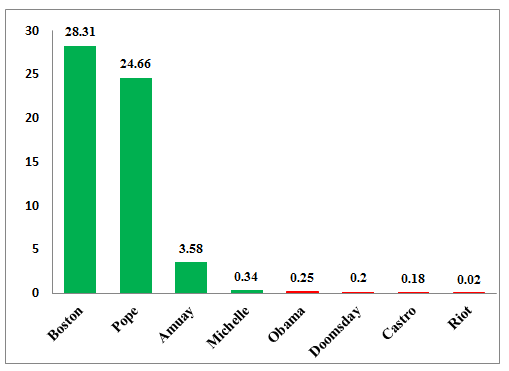
\includegraphics[width=4in]{pictures/reproductive-ratio.png}
   \caption{$R_{SI}$ values for eight Twitter datasets.}
  \label{fig:ratio}
\end{figure}


We then computed $R_{SI}$ using the specific parameter values attained from our model fits of the eight cases (Figure~\ref{fig:ratio}).
%, and examined these values (Table ~\ref{table:SEIZ-parameter}).
Here we can see that the true news about the Boston Marathon bombing, Pope resignation, and Amuay refinery explosion do in fact have much higher $R_{SI}$ values than the rumor topics: Doomsday, Fidel Castro death, Mexico City riots, and Barrack Obama injury which each have much lower $R_{SI}$ values. However, the Michelle presence at the Oscars, which is classified as true news, has a very low $R_{SI}$ value. This particular case is interesting since Michelle did not really show up to the 2013 Oscar Awards Ceremony. She simply participated remotely via video telecast. It is thus arguable that this topic could
have been discussed in the media in terms similar to rumors.

These findings suggest, for these specific topics, that the parameters in the SEIZ model can potentially aid in the challenge of distinguishing rumor versus true news. We are not claiming that the $R_{SI}$ value is the unique measure to accomplish this, nor are we claiming that the SEIZ model itself is the sole tool to do this. As is suggested by our findings, we postulate that a fit of a compartmental model, in the spirit of the SEIZ model, to Twitter data provides valuable propagation information that can be coupled with other data analysis strategies  (e.g., content modeling)
to augment the accuracy and reliability of true news story and rumor topic discrimination.

%As we can see from the figures, all $S$ will be zero ultimately because the slope of $S$ is always negative, as shown in the equation (2-a)\ycaoc{again, use ref}. This can be explained by an assumption that given an infinite time, every tweet user should hear about a particular piece of news. For the same reason, the $E$ will also be zero ultimately. When its slope is zero, $E$ reaches its maximal value, denotes as $E_{max}$. At this point, we have an equation from Figure 5\ycaoc{again, use ref command here. Another question is: are you sure this equation is from Figure 5, not Equaqtion 2b? It seems to me that Equation 2b is a better source to derive this equation.}
%$$(1-p)\beta S+(1-l)bS=E(\rho + \epsilon).$$
%%This is because its inputs should be equal to its outputs.
%
%Obviously, a bigger $E_{max}$ value indicates more tweet users who used to be exposed and later be infected. Since at this point, $E$ has its maximal value, which will also turn into the infected and post tweets. While at this point, the $S$ means the users who still have not heard about this tweet news, but at last they will hear about this news\ycaoc{I don't understand these sentences here. Some changes should be made.}. Thus, we use the the ratio of $E$ to $S$ as $$R_{ES}=\frac{(1-p)\beta +(1-l)b}{\rho + \epsilon}$$ to measure the transition of those users.
%
%Table~\ref{table:SEIZ-parameter} lists the SEIZ model parameters for the studied Twitter data. Here we set the threshold as 1, if the ratio  $R_{ES}$ of a news is higher than 1, we assume that it is a ``truth", otherwise, we suspect that it is a ``rumor". We can see that news about Boston, Pope, Mexico, and Amuay explosion have much higher $R_{ES}$ values, while Obama injured, Doomsday, and Fidel Castro rumors have much lower $R_{ES}$ values. An interesting case lies in the Twitter data for Michelle's appearance in Oscar, which though has a ratio higher than the three rumors, still is quite close to a rumor, because the $E$ doesn't change much. Actually, Michelle did not really show up in the 2013 Oscar but just participated remotely by video signals. Thus, one may argue that this news is a rumor.
%
%The difference between the SEIZ model and the SIS model is that the SEIZ model introduces the $E$ status to represent users who know about the news but take some time before posting anything about it. Usually, when some real news happen, people don't get the verified information, thus the $E$ value will increase, because at this time many people have an ambiguous attitude and don't post tweets. But after some time, when people get some verified information, those exposed people will become infected and post tweets, and thus the $E$ value will decrease sharply. So, if the $E$ curve increases first, and then decreases, then it is highly possible that this is a truth.

%Taking the Boston news tweet data for example, we can see from figure~\ref{fig:boston_time_course} that the \textbf{E} peaks at time time 20. At this time many people were exposed to this news, but were not ``infected", because they have an ambiguous attitude about this tweet news. However, after that $E$ decreases sharply, which indicates that those people changed their attitude, and were ``infected". This is probably because people got some proven information about this new, and those exposed people began to post tweets. We can also see that the Pope and Gas tweet news have the same feature, thus we can consider them as real news. However, from the figures for the Doomsday and Castro rumors, we can see that the curve of $E$ is always low, because people can not get any verified information about those news. Thus, it is highly possible that those tweets are just rumors.
